\ZbSec{Flutter}
Um Flutter zu installieren, bestehen verschieden Optionen. Hierbei werde ich näher auf die manuelle Installation und die Installation per Chocolatey eingehen. Die manuelle Installation ist etwas aufwendiger als die Installation per choco, da man bei der manuellen Installation noch den Pfad setzten muss, was bei choco erspart bleibt. (vgl. \cite{FlutterInstall})
\begin{itemize}
    \item \textbf{Chocolatey}: (vgl. \cite{Choco})
    \begin{enumerate}
        \item Install choco: Folgenden Befehl in ein Terminal mit Admin Rechten einfügen: 
        \begin{lstlisting}[style=flutterListingStyle,caption={Choco installieren}] 
        Set-ExecutionPolicy Bypass -Scope Process -Force; [System.Net.ServicePointManager]::SecurityProtocol = [System.Net.ServicePointManager]::SecurityProtocol -bor 3072; iex ((New-Object System.Net.WebClient).DownloadString('https://community.chocolatey.org/install.ps1'))\end{lstlisting}
        \item Install Flutter: \textbf{choco install flutter -y}
        \item Zuletzt noch \textbf{flutter doctor} in einem Terminal laufen lassen. Vor dem Eintrag Android Studio sollte sich ein grüner Haken befinden. Die anderen Einträge können ignoriert werden.
    \end{enumerate}

    \item \textbf{Manuell}:
    \begin{enumerate}
        \item ZIP Datei von Flutter herunterladen: \href{https://storage.googleapis.com/flutter_infra_release/releases/stable/windows/flutter_windows_3.7.3-stable.zip}{Flutter Download}.
        \item Diese ZIP Datei nach C:\textbackslash src\textbackslash flutter entpacken
        \item Pfad Variablen setzten: In Windows suche System variablen eingeben, danach auf – Environment Variables – Benutzer variablen – Pfad – Edit drücken. Danach dort einen neuen Eintrag einfügen mit dem Pfad zu Flutter\textbackslash bin z. B.: C:\textbackslash tools\textbackslash flutter\textbackslash bin und dann ``OK`` drücken. Hier folgt die bildnerische Beschreibung:
        \begin{figure}[!h]
        \vspace{0.5cm}
        \centering
        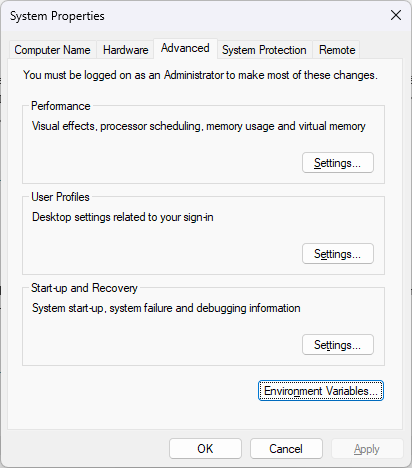
\includegraphics[width=0.6\textwidth]{FLUTTER/images/ZB/flutter_path_variable.png}
        \caption{System Variablen anpassen}
        \end{figure}
        \begin{figure}[!h]
        \centering

        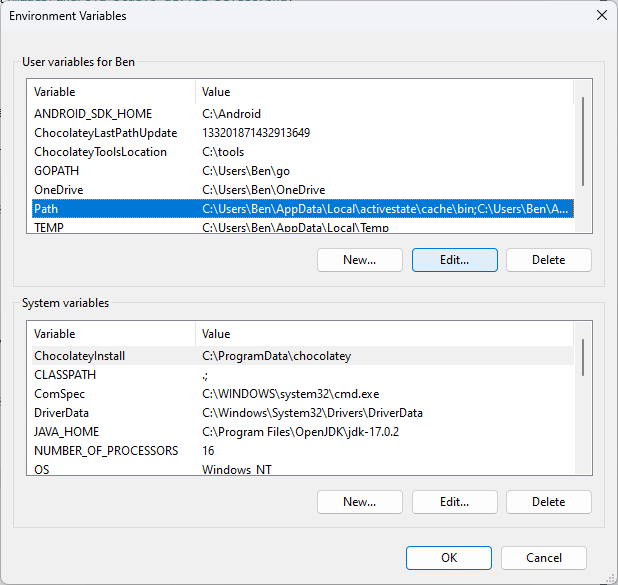
\includegraphics[width=0.5\textwidth]{FLUTTER/images/ZB/flutter_path_variable_edit.png}
        \caption{Path bearbeiten}
        \end{figure}
        \begin{figure}[!h]
        \centering
        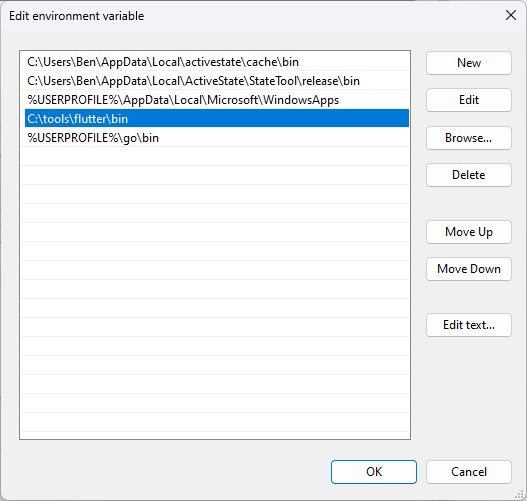
\includegraphics[width=0.5\textwidth]{FLUTTER/images/ZB/flutter_path_variable_add.png}
        \caption{Eintrag einfügen}
        \end{figure}
        
        \item Zuletzt noch \textbf{flutter doctor} in einem Terminal ausführen. Vor dem Eintrag Flutter sollte ein grüner Haken sein. Die anderen Einträge können ignoriert werden.
    \end{enumerate}
\end{itemize}


\ZbSec{Android Studio}
\subsection{Installation}
Selbiges Spiel auch hier. Es besteht die Möglichkeit Android Studio über einen Installer oder Chocolatey zu installieren. Choco funktioniert auch hier einfacher und schneller. (vgl. \cite{Android-Studio})
\begin{itemize}
    \item \textbf{Chocolatey}:
    \begin{enumerate}
        \item Install Flutter: \textbf{choco install androidstudio -y}
        \item Zuletzt noch \textbf{flutter doctor} in einem Terminal laufen lassen. Vor dem Eintrag Android Studio sollte sich ein grüner Haken befinden. Die anderen Einträge können ignoriert werden.
    \end{enumerate}
    
    \item \textbf{Manuell}:
    \begin{enumerate}
        \item Installer von Android Studio herunterladen: \href{https://redirector.gvt1.com/edgedl/android/studio/install/2022.1.1.20/android-studio-2022.1.1.20-windows.exe}{Android Studio Download}.
        \item Diese Datei dann wie bei allen andern Programmen doppelklick auf die Datei und dem Installer folgen.
        \item Zuletzt noch Flutter doctor in einem Terminal laufen lassen. Vor dem Eintrag Android Studio sollte sich ein grüner Haken befinden. Die anderen Einträge können ignoriert werden.
    \end{enumerate}
\end{itemize}

\newpage

\subsection{Emulator erstellen }
Um einen Emulator erstellen zu können. Erstmals Android Studio öffnen. Wenn dies das erste Mal ist, werden ein paar Fragen gestellt und womöglich die Android SDK installiert. Wenn dies getan ist, danach, More Actions öffnen und auf Virtual Device Manager klicken. 
\begin{figure}[!h]
\centering
\vspace{0.5cm}
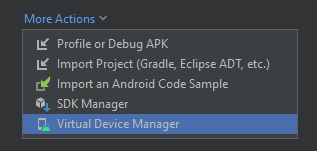
\includegraphics[width=0.5\textwidth]{FLUTTER/images/ZB/android_studio.png}
\caption{Android Studio}
\end{figure}

Danach Gerät erstellen klicken
\begin{figure}[!h]
\centering
\vspace{0.5cm}
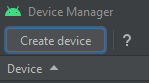
\includegraphics[width=0.5\textwidth]{FLUTTER/images/ZB/android_studio_add_device.png}
\caption{Neuen Emulator anlegen}
\end{figure}

Hier wird dann, wenn Emulatoren vorhanden sind, diese angezeigt. Des Weiteren dann in der linken oberen Ecke auf Create Device klicken. Wie im Bild gezeigt, ein Gerät auswählen und dann auf weiter drücken. Es ist per se egal, welches Gerät gewählt wird, die App kann mit allen verwendet werden.
\begin{figure}[!h]
\centering
\vspace{0.5cm}
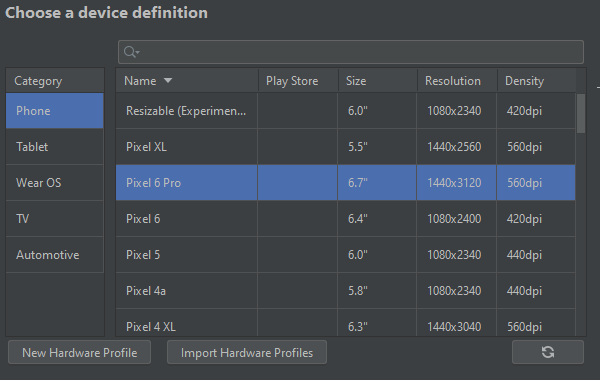
\includegraphics[width=0.65\textwidth]{FLUTTER/images/ZB/android_studio_device_select.png}
\caption{Gerät auswählen}
\end{figure}

Nun sollte die Android Version ausgewählt werden. Zur Entwicklung verwendeten wir \textbf{API Level 33}. Diese Option auswählen. Falls dies nicht vorhanden sein sollte ``Download`` drücken und installieren. Nun sollte es folgendermaßen aussehen:
\begin{figure}[!h]
\vspace{0.5cm}
\centering
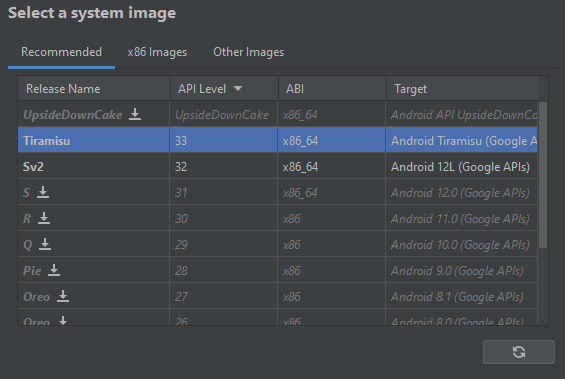
\includegraphics[width=0.65\textwidth]{FLUTTER/images/ZB/android_studio_version_select.png}
\caption{API Version auswählen}
\end{figure}

Drücken Sie danach einfach noch auf ``Weiter`` und klicken Sie auf der nächsten Seite auf ``Fertigstellen``. Somit wurde der Emulator erfolgreich erstellt. Nun sollte ein neuer Emulator angelegt worden sein.
\begin{figure}[!h]
\centering
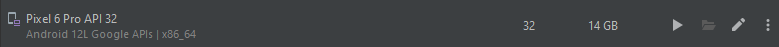
\includegraphics[width=1\textwidth]{FLUTTER/images/ZB/android_studio_devices.png}
\caption{Emulatoren}
\end{figure}

\newpage

\ZbSec{Docker}
\subsection{Installation}
Selbiges Spiel auch hier. Es besteht die Möglichkeit Docker über einen Installer oder Chocolatey zu installieren. (vgl. \cite{Docker})
\begin{itemize}
    \item \textbf{Chocolatey}:
    \begin{enumerate}
        \item Install Docker: \textbf{choco install docker-desktop -y}
        \item Danach WSL installieren. Diesen Befehl und auch den nächsten in einem Admin Terminal ausführen: \textbf{WSL --install}
        \item Weiters die Version von WSL für Docker auf 2 setzten: \textbf{ wsl --set-version docker-desktop 2}
        \item Docker ist dann bereits verwendbar
    \end{enumerate}

    \item \textbf{Manuell}:
    \begin{enumerate}
        \item Installer von Docker Desktop herunterladen: \href{https://desktop.docker.com/win/main/amd64/Docker%20Desktop%20Installer.exe}{Docker Desktop Download}.
        \item Diese Datei dann wie bei allen andern Programmen doppelklick auf die Datei und dem Installer folgen.
        \item Danach WSL installieren. Diesen Befehl und auch den nächsten in einem Admin Terminal ausführen: \textbf{WSL --install}
        \item Weiters die Version von WSL für Docker auf 2 setzten: \textbf{ wsl --set-version docker-desktop 2}
        \item Danach ist Docker voll verwendbar.
    \end{enumerate}
\end{itemize}

\newpage

\subsection{API – starten}
Nähere Informationen zur Konfiguration der zentralen Schnittstelle sowie den Simulatoren finden sich einerseits in der Implementierung (Abschnitt \ref{sec:impl:simulators}) sowie dem entsprechenden Abschnitt im Benutzerhandbuch (\ref{sec:apdx:user-guide:mj}). 

\subsubsection{Container starten}
Erster Schritt, ein Terminal aufrufen, in das Git Repo klonen und zum Branch \texttt{golang\_Api} wechseln. Hier im Terminal dann den command: \textbf{\texttt{docker compose up -{}-build}} eingeben und enter drücken. Hiermit wird dann der Container gebuilded und gestartet.

\subsubsection{Controller Simulator – starten}
Um dann noch mit Storages testen zu können, muss der Controller gestartet werden. Dazu in \texttt{golang\_Api} zu \texttt{api/simulator/controller} wechseln. Dort dann \textbf{\texttt{go run controller.go -{}-client-id Storage1 -{}-topic S1@L1/1}} ausführen. Die client-id und das topic können beliebig gewählt werden. Wenn mehrere Storages benutzt werden sollen, einfach ein neues Terminal öffnen und diese Schritte wiederholen.

\subsubsection{Client Simulator – starten}
Wenn noch Karten, Storages etc. angelegt werden sollen, muss der Client Simulator gestartet werden. Dieser befindet sich in \texttt{api/simulator/client}. Dort einfach \textbf{go run .} ausführen und der Simulator wird gestartet. Damit man dort Aktionen ausführen kann, muss der Benutzer authentifiziert werden. Einfach \textbf{21} (Code um einen Benutzer zu authentifizieren) eingeben und die konfigurierte Administrator-E-Mail-Adresse, standardmäßig \textbf{card\_storage\_admin@default.com}, eingeben. Der Client hat nun Admin Rechte und kann alle Aktionen ausführen.
\medskip
Nun ist die API einsatzfähig.

\newpage

\ZbSec{VS Code }
\subsection{Installation}
Selbiges Spiel auch hier. Es besteht die Möglichkeit Visual Studio Code über einen Installer oder Chocolatey zu installieren. Choco funktioniert auch hier einfacher und schneller. (vgl. \cite{VS-Code-Install})
\begin{itemize}
    \item \textbf{Chocolatey}:
    \begin{enumerate}
        \item Install VS Code: \textbf{choco install vscode -y}
        \item Zuletzt noch \textbf{flutter doctor} in einem Terminal laufen lassen. Vor dem Eintrag VS Code sollte sich ein grüner Haken befinden. Die anderen Einträge können ignoriert werden.
    \end{enumerate}
    
    \item \textbf{Manuell}:
    \begin{enumerate}
        \item Installer von VS Code herunterladen: \href{https://code.visualstudio.com/docs/?dv=win}{VS Code Download}.
        \item Diese Datei dann wie bei allen andern Programmen doppelklick auf die Datei und dem Installer folgen.
        \item Zuletzt noch Flutter doctor in einem Terminal laufen lassen. Vor dem Eintrag VS Code sollte sich ein grüner Haken befinden. Die anderen Einträge können ignoriert werden.
    \end{enumerate}
\end{itemize}

\newpage

\subsection{Extensions}
Um Flutter Entwicklung mit VS Code durchführen zu können, sollte man sich 2 Extensions installieren. Die erste wäre Flutter und die zweite Dart. Diese kann man über den Reiter Extensions installieren. Dort nach den jeweiligen Extensions suchen und installieren drücken.

\begin{figure}[!h]
\centering
\vspace{0.5cm}
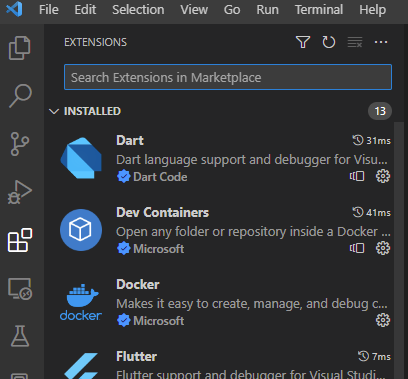
\includegraphics[width=1\textwidth]{FLUTTER/images/ZB/vscode_extensions.png}
\caption{Extensions}
\end{figure}

\newpage

\subsection{Emulator aufrufen}
Um einen Emulator starten zu können, muss dieser zuerst erstellt werden, wie im Abschnitt Emulator erstellen beschrieben ist. Wenn dies getan wurde VS Code öffnen, den Code der App laden und unten rechts wo Windows steht klicken:

\begin{figure}[!h]
\centering
\vspace{0.5cm}
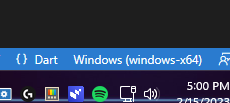
\includegraphics[width=0.7\textwidth]{FLUTTER/images/ZB/emulator_selector.png}
\caption{Emulator starten}
\end{figure}

Danach in der Liste, welche sich am oberen Rand in der Mitte öffnet, den jeweiligen Emulator öffnen:
\begin{figure}[!h]
\centering
\vspace{0.5cm}
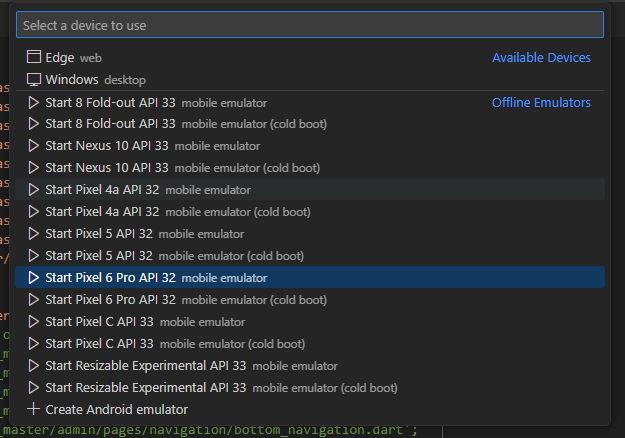
\includegraphics[width=0.7\textwidth]{FLUTTER/images/ZB/emulator_auswaehlen.png}
\caption{Emulator auswählen}
\end{figure}

\newpage

Wenn dies getan wurde, sollte am Bildschirm ein Emulator geöffnet werden:
\begin{figure}[!h]
\centering
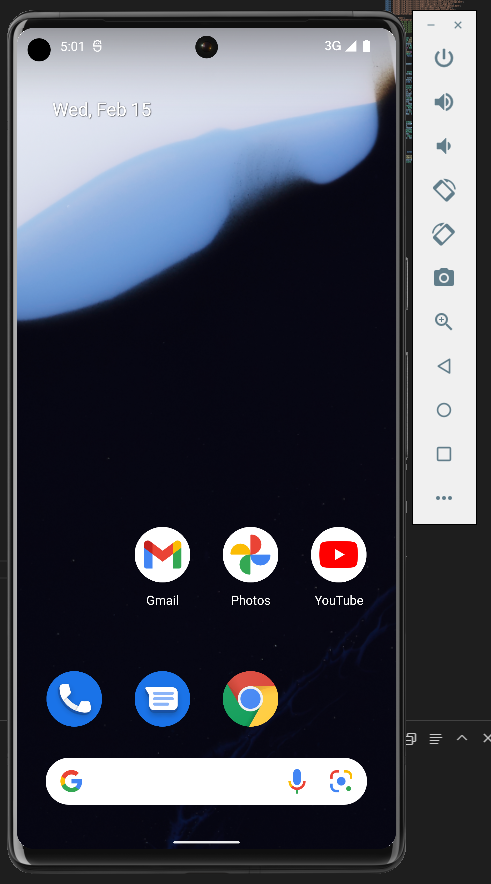
\includegraphics[width=0.3\textwidth]{FLUTTER/images/ZB/gestartetter_emulator.png}
\caption{Emulator}
\end{figure}

\subsection{App Starten}
Um die App zu Starten muss lediglich der Emulator geöffnet werden, wie vorher beschrieben. Danach die main.dart Datei öffnen und rechts oben in der Leiste das Play Icon drücken:

Wenn dies getan wurde, sollte am Bildschirm ein Emulator geöffnet werden:
\begin{figure}[!h]
\centering
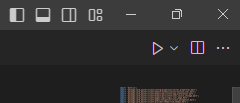
\includegraphics[width=0.3\textwidth]{FLUTTER/images/ZB/start_emulator.png}
\caption{Start App mit Emulator}
\end{figure}

Nun kann man ohne weiteres mit der Entwicklung beginnen.

\newpage

\ZbSec{Anpassung visueller Auftritt }

\subsubsection{App Name}
Der App Name kann sehr einfach geändert werden. Dazu muss lediglich die pubspec.yaml geöffnet werden. Dort lässt sich ein Eintrag finden, welcher flutter\_app\_name heißt. (vgl. \cite{AppName})

\vspace{0.5cm}
\begin{lstlisting}[style=flutterListingStyle,caption={App Name ändern}] 
flutter_app_name:
  name: "Card Master"
\end{lstlisting}

Wenn der Name gesetzt wurde, in einem Terminal diesen Command ausführen:
\vspace{0.5cm}
\begin{lstlisting}[style=flutterListingStyle,caption={App Name ändern},label={lst:appNameSetzen}] 
flutter pub run flutter_app_name
\end{lstlisting}

\newpage

\subsubsection{App Icon}
Das App Icon lässt sich auf praktisch gleicherweise ändern. Dazu muss lediglich die pubspec.yaml geöffnet werden. Dort lässt sich ein Eintrag finden, welcher flutter\_icons heißt. Dort wird angegeben, für welche Plattform das Icon verwendet werden soll und wo es sich befindet. (vgl. \cite{AppIcon})

\vspace{0.5cm}
\begin{lstlisting}[style=flutterListingStyle,caption={App Icon ändern},label={lst:appIcon}] 
flutter_icons:
  image_path: "assets/icon.png"
  android: true
  ios: true
\end{lstlisting}

Danach sollte man in dem Ordner assets ein Bild mit dem vorher angegebenen Namen ablegen. 

Danach besucht man folgende Webseite https://appicon.co/. Dort wählt man Android und IOS aus und drückt auf Generate. 
\begin{figure}[!h]
\centering
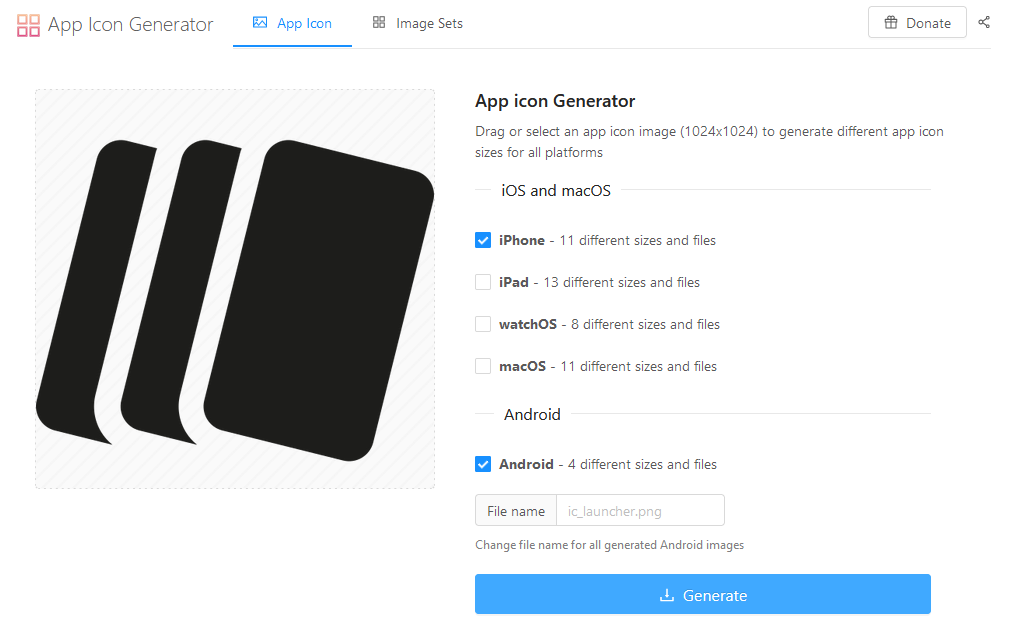
\includegraphics[width=0.7\textwidth]{FLUTTER/images/ZB/download_app_icon.png}
\caption{Icon herunterladen}
\end{figure}

\newpage

Die Heruntergeladene ZIP-Datei entpackt man dann. Der Inhalt sollte folgendes sein:
\begin{figure}[!h]
\centering
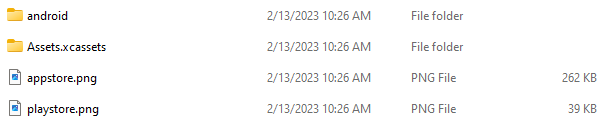
\includegraphics[width=0.65\textwidth]{FLUTTER/images/ZB/downloaded_files.png}
\caption{Heruntergeladene Files}
\end{figure}

Als erstes kopiert man alle Dateien im android Ordner. Folgende Dateien:
\begin{figure}[!h]
\centering
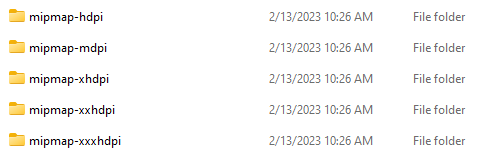
\includegraphics[width=0.65\textwidth]{FLUTTER/images/ZB/downloaded_android_icons.png}
\caption{Dieses Files kopieren}
\end{figure}

Danach wechselt man zu folgendem Pfad: android/app/src/main/res. Dort fügt man die vorher kopierten Ordner ein. Ersetzten auswählen und Fertig für Android.
\begin{figure}[!h]
\centering
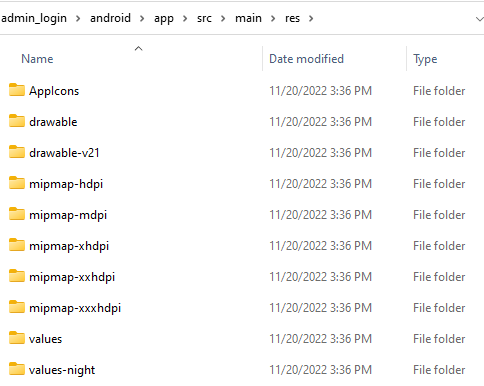
\includegraphics[width=0.65\textwidth]{FLUTTER/images/ZB/android_icons_copy_to.png}
\caption{Android Files in diesen Ordner kopieren}
\end{figure}

\newpage

Als Nächstes kopieren wir aus unseren heruntergeladenem Dateien Assets.xcassets.
\begin{figure}[!h]
\centering

\includegraphics[width=0.7\textwidth]{FLUTTER/images/ZB/downloaded_ios_icons.png}
\caption{Dieses Files kopieren}
\end{figure}

Danach wechselt man zu folgendem Pfad: ios/Runner/Assets.xcassets. Dort fügt man den vorher kopierten Ordner ein. Ersetzten auswählen und fertig für IOS.
\begin{figure}[!h]
\centering
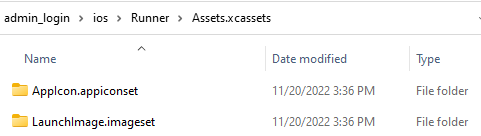
\includegraphics[width=0.7\textwidth]{FLUTTER/images/ZB/ios_icons_copy_to.png}
\caption{IOS Files in diesen Ordner kopieren}
\end{figure}

\newpage

\subsubsection{Lade Bildschirm}
Um den Lade Bildschirm zu ändern, muss man lediglich die Bilddatei tauschen und den Namen des Bildes im Code ändern. In der Ordnerstruktur der App findet sich ein {\textit{img}} Ordner. In den fügt man das gewünschte Bild ein. In der Splashscreen Datei sucht man sich dann diese Zeile: (vgl. \cite{SplashScreen})

\vspace{0.5cm}
\begin{lstlisting}[caption=Dateiname anpassen und die größe]

\end{lstlisting}
\begin{lstlisting}[style=flutterListingStyle,caption={App Icon importieren},label={lst:appIconSetzen}] 
Image.asset("img/splashscreen.jpg", height: 200.0, width: 200.0)
\end{lstlisting}
Hier muss nur den Dateinamen anpassen und gegebenenfalls die Größe des Bildes.

\newpage

\GpSec{Generierung der Flutter-APK-Datei }
Um die Applikation nun auf einem Android-Gerät laufen zu lassen, wird das Flutter Projekt in eine APK {\textit{Android Package Kit}} umgewandelt. Eine APK enthält alle Dateien, die nötig sind, um die Anwendung auf dem Smartphone zu benutzen. (vgl. \cite{Generierung-AppBundle})

Ablauf der Generierung einer APK:
\begin{itemize}
    \item Zunächst wechseln Sie in das Stammverzeichnis {\textit{/CARD\_MASTER}}
    \item Öffnen Sie das Terminal und kopieren Sie den Befehl: {\textbf{flutter build apk --release}}
    \item Nach Fertigstellung, finden Sie die APK unter {\textit{/build/app/outputs/flutter-apk/app-release.apk}}.
    \item Um die APK vom Computer auf ein Android-Gerät zu laden, können Sie diese über einen Server oder per E-Mail an die gewünschte(n) Person(en) zur Verfügung stellen.
    \item Die Installation am Android-Gerät erfolgt per Klick auf die APK – Fertig 
\end{itemize}

\GpSec{Flutter Bundle f\"ur Raspberry Pi}
Um die Flutter Anwendung, für das Display am Tresor zu verwenden, wird {\textbf{Flutter-pi}} verwendet. Flutter-pi ist ein Open-Source-Projekt, welche die Ausführung der Flutter Anwendungen am Raspberry Pi ermöglicht. (vgl. \cite{Flutter-Pi})

Anleitung zur Installation von Flutter-pi am Raspberry:\\
{\textbf{Voraussetzung:}} Raspberry Pi mit installiertem Raspberry OS und angeschlossenem Display

\newpage

\begin{itemize}
    \item {\textbf{Schritt 1:}} Installation der {\textit{flutter engine binaries}} 
    \begin{lstlisting}[style=flutterListingStyle, caption=Installation flutter engine binaries]
git clone --depth 1 https://github.com/ardera/flutter-engine-binaries-for-arm.git engine-binaries
cd engine-binaries
sudo ./install.sh
\end{lstlisting}
\item {\textbf{Schritt 2:}} Installieren verschiedener Assets
    \begin{lstlisting}[style=flutterListingStyle, caption=Installation Bibliotheken]
sudo apt install cmake libgl1-mesa-dev libgles2-mesa-dev libegl1-mesa-dev libdrm-dev libgbm-dev ttf-mscorefonts-installer fontconfig libsystemd-dev libinput-dev libudev-dev  libxkbcommon-dev
\end{lstlisting}
\item {\textbf{Schritt 3:}} Aktualisierung der Systemschriftarten 
\begin{lstlisting}[style=flutterListingStyle, caption=Aktualisierung der Systemschriftarten ]
sudo fc-cache
\end{lstlisting}
\item {\textbf{Schritt 4:}} Installation von flutter-pi
\begin{lstlisting}[style=flutterListingStyle,caption=Installation von flutter-pi]
git clone https://github.com/ardera/flutter-pi
cd flutter-pi
\end{lstlisting}
\item {\textbf{Schritt 5:}} Kompilieren und Installieren Sie flutter-pi 
\begin{lstlisting}[style=flutterListingStyle,caption=Kompilieren flutter-pi]
mkdir build && cd build
cmake ..
make -j`nproc`
sudo make install
\end{lstlisting}
\item {\textbf{Schritt 6:}}  Öffnen der Raspberry Einstellungen mit
\begin{lstlisting}[style=flutterListingStyle,caption=Einstellungen Raspberry]
sudo raspi-config
\end{lstlisting}

\item {\textbf{Schritt 7:}} Gehen Sie unter {\textit{System Options → Boot/Auto Login}} und w\"ahlen Sie Console oder Console Autologin aus
\begin{figure}[!h]
        \centering
        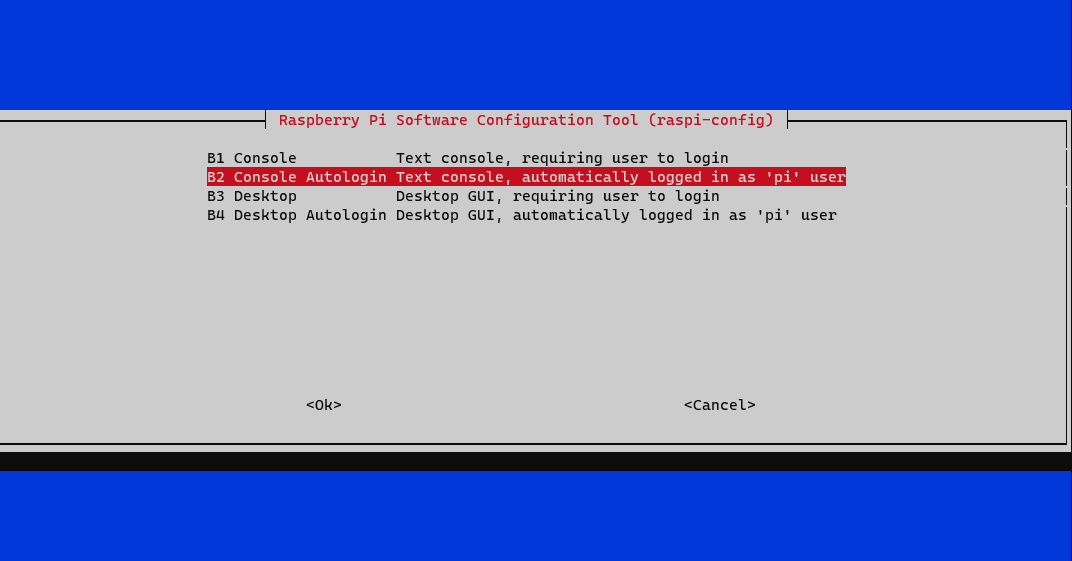
\includegraphics[width=0.7\textwidth]{FLUTTER/images/GP/raspberry_autologin.png}
        \caption{Raspberry Autologin}
        \end{figure}
    
\item {\textbf{Schritt 8:}} V3D graphics Treiber aktivieren unter (Nur für Raspberry Pi 3){\textit{Advanced Options → GL Driver → GL (Fake KMS)}}
\newpage

\newpage

\item {\textbf{Schritt 9:} Einstellen des Grafik speichers unter \textit{Performance Options → GPU Memory} und 64 MB zuweisen}
\begin{figure}[!h]
        \vspace{0.5cm}
        \centering
        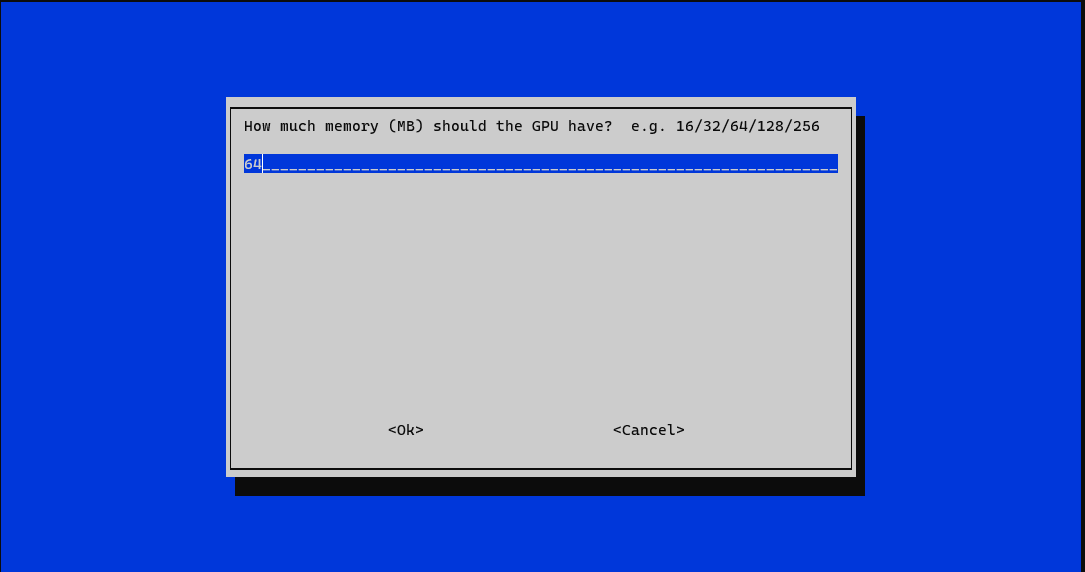
\includegraphics[width=1\textwidth]{FLUTTER/images/GP/raspberry_gpumemory.png}
        \caption{Änderung des Grafikspeichers auf 64 MB}
        \end{figure}
\item {\textbf{Schritt 10:}} Einstellungen des Raspberry mit ESC verlassen
\item {\textbf{Schritt 11:}} Neustart des Raspberrys mit 
\begin{lstlisting}[style=flutterListingStyle,caption=Neustart]
sudo reboot
\end{lstlisting}
\end{itemize}
Wenn alles korrekt abgelaufen ist, kann die Flutter Anwendung am Raspberry kompiliert werden. Wechseln Sie daher auf Ihren Rechner, und öffnen Sie das Flutter Projekt.\\

\newpage

Der Ablauf, um eine Flutter Anwendung an den Raspberry zu senden:

\begin{itemize}
\item {\textbf{Schritt 1:}} Zunächst werden alle generierten und temporären Dateien vom Projektverzeichnisses entfernt:
\begin{lstlisting}[style=flutterListingStyle,caption=Flutter clean]
flutter clean
\end{lstlisting}

\item {\textbf{Schritt 2:}} Danach wird eine {\textit{Bundle Datei}} erzeugt. Eine Bundle-Datei enth\"ahlt alle Ressourcen und Assets, die zum Start der Anwendung benötigt werden.
\begin{lstlisting}[style=flutterListingStyle,caption= Bundle erstellen]
flutter build bundle
\end{lstlisting}

\item {\textbf{Schritt 3:}} Nun muss das erstellte \textit{Bundle} an den Raspberry gesendet werden. In diesem Fall verwenden wir Scp. Scp ermöglicht den Datentransfer zwischen zwei Rechnern.
\begin{lstlisting}[style=flutterListingStyle,caption=Senden der Datei]
scp -r ./build/flutter_assets pi@<ip_address_of_reTerminal>:/home/pi/testapp
\end{lstlisting}
\end{itemize}

\vspace{0.5cm}
Das Bundle kann nun am Raspberry mit diesem Befehl kompiliert und angezeigt werden.
\begin{lstlisting}[style=flutterListingStyle]
flutter-pi /home/pi/testapp
\end{lstlisting}